% !TEX TS-program = pdflatex
% !TEX encoding = UTF-8 Unicode

% This is a simple template for a LaTeX document using the "article" class.
% See "book", "report", "letter" for other types of document.

\documentclass[11pt]{article} % use larger type; default would be 10pt

\usepackage[utf8]{inputenc} % set input encoding (not needed with XeLaTeX)
\usepackage{gensymb}
\usepackage[hidelinks]{hyperref}
%%% Examples of Article customizations
% These packages are optional, depending whether you want the features they provide.
% See the LaTeX Companion or other references for full information.

%%% PAGE DIMENSIONS
\usepackage{geometry} % to change the page dimensions
\geometry{a4paper} % or letterpaper (US) or a5paper or....
% \geometry{margin=2in} % for example, change the margins to 2 inches all round
% \geometry{landscape} % set up the page for landscape
%   read geometry.pdf for detailed page layout information

\usepackage{graphicx} % support the \includegraphics command and options
\usepackage{wrapfig}
 \usepackage[font=footnotesize,labelfont=bf]{caption} %changes caption size
% \usepackage[parfill]{parskip} % Activate to begin paragraphs with an empty line rather than an indent

%%% PACKAGES
\usepackage{booktabs} % for much better looking tables
\usepackage{array} % for better arrays (eg matrices) in maths
\usepackage{paralist} % very flexible & customisable lists (eg. enumerate/itemize, etc.)
\usepackage{verbatim} % adds environment for commenting out blocks of text & for better verbatim
\usepackage{subfig} % make it possible to include more than one captioned figure/table in a single float
% These packages are all incorporated in the memoir class to one degree or another...

%%% HEADERS & FOOTERS
\usepackage{fancyhdr} % This should be set AFTER setting up the page geometry
\pagestyle{fancy} % options: empty , plain , fancy
\renewcommand{\headrulewidth}{0pt} % customise the layout...
\lhead{}\chead{}\rhead{}
\lfoot{}\cfoot{\thepage}\rfoot{}

%%% SECTION TITLE APPEARANCE
\usepackage{sectsty}
\allsectionsfont{\sffamily\mdseries\upshape} % (See the fntguide.pdf for font help)
% (This matches ConTeXt defaults)

%%% ToC (table of contents) APPEARANCE
\usepackage[nottoc,notlof,notlot]{tocbibind} % Put the bibliography in the ToC
\usepackage[titles,subfigure]{tocloft} % Alter the style of the Table of Contents
\renewcommand{\cftsecfont}{\rmfamily\mdseries\upshape}
\renewcommand{\cftsecpagefont}{\rmfamily\mdseries\upshape} % No bold!

%%% END Article customizations

%%% The "real" document content comes below...


\date{} % Activate to display a given date or no date (if empty),
         % otherwise the current date is printed 
\title{Glucocorticoid-Induced Metabolic Disturbances are Exacerbated in
Obesity}

\author{Innocence Harvey, Erin J. Stephenson, JeAnna R. Redd,\\ Quynh T. Tran,
Irit Hochberg, Nathan Qi and Dave Bridges\footnote{Please address any correspondance to \href{mailto:davebrid@umich.edu}{davebrid@umich.edu}}}

\begin{document}
\maketitle

\abstract{
Obesity and chronically elevated glucocorticoids result in similar
co-morbidities, but the effect of a combination of these ailments on
metabolic outcomes is unclear. Measures of glucose homeostasis and
markers of hepatic lipid accumulations were assessed to determine
whether obesity exaggerated the effects of dexamethasone-induced
metabolic disturbances. The combination of obesity and glucocorticoids
resulted in synergistic elevations in hepatic steatosis and insulin
resistance and this was matched with synergistic elevations in markers
of lipolysis. These findings suggest lipolysis may be a key player in
glucocorticoid-induced insulin resistance and fatty liver in people with
obesity.}

\section*{Introduction }

Cushing's syndrome is an endocrine disorder that manifests in response
to chronically elevated levels of glucocorticoids and is often
associated with changes in adipose mass and distribution (1), fatty
liver (2,3), impaired glucose tolerance and type 2 diabetes (4,5).
Although prevalence of Cushing's syndrome is rare, it is estimated that
at any given time 1-3\% of the US, UK and Danish populations are
prescribed exogenous corticosteroids, which may increase their risk for
developing some of the same metabolic complications observed in
Cushing's syndrome (6--9).

Similarly to Cushing's syndrome, Obesity is often accompanied by a
multitude of metabolic complications, such as insulin resistance
(10--12) and NAFLD (13,14) and is becoming a worldwide epidemic.
Comparing the increased levels/amounts of corticosteroid prescription
with the prevalence of overweight and obesity in developed countries, it
is likely that the combination of obesity and glucocorticoid excess is
present in many individuals; though, to our knowledge, this has not been
studied.

Given the similar co-morbidities associated with obesity and chronically
elevated glucocorticoids, we hypothesized that the combinations of these
two conditions would lead to worse metabolic outcomes than either of
them alone. This is supported by studies in rats showing that
corticosterone and high-fat diets combine to cause worsened insulin
resistance and non-alcoholic fatty liver disease (NAFLD; (15,16)).
However, the underlying mechanisms remain unclear.

There is an array of physiological changes that occur as a result of
elevated glucocorticoids including decreased lean mass (17--19),
increased fat mass (18,20,21) and increased lipolysis (22--24), all of
which have been associated with decreased insulin sensitivity (25--27).
Likewise, obesity, insulin resistance and increased fatty acid flux are
associated with NAFLD (13,28--30). It has also been demonstrated that
inhibition of lipolysis promotes insulin sensitivity (25,31--33). Recent
tissue-specific knockouts of glucocorticoid signaling molecules have
implicated adipose tissue as a central node linking glucocorticoid
action and lipolysis to systemic insulin resistance and NAFLD (34--37).

Here, we show that chronically elevated glucocorticoids in the presence
of obesity have synergistic effects on lipolysis, insulin resistance and
fatty liver disease. Obese glucocorticoid-treated mice have reduced fat
mass compared to all other groups, yet have hyperglycemia and severe
insulin resistance; therefore, we speculate that lipolysis drives
insulin resistance in obese animals.

\section*{Methods}

\textbf{Patient Recruitment and data collection}: Written informed
consent was obtained and the study was approved by the internal review
board of the University of Michigan Medical System. All procedures
follow the Helsinki declaration. Patients undergoing transsphenoidal
adenomectomy at the University of Michigan were recruited and data was
collected as described in Hochberg et al. (18). Control patients were
those that had non-secreting adenomas and Cushing's patients were those
that had ACTH-secreting adenomas.

\textbf{Animal Procedures:} C57BL/6J adult male mice were purchased from
the Jackson Laboratory at nine weeks of age. All animals were on a light
dark cycle of 12/12hrs and housed at 22\degree C. Following a week of
acclimation, chow-fed 12-week dexamethasone-treated mice were treated as
described previously (18). Additional cohorts of mice used in these
experiments either remained on a standard diet (normal chow diet; NCD;
5L0D LabDiet; 13\% fat; 57\% carbohydrate; 30\% protein) or were
provided a high fat diet (45\% fat from lard; 35\% carbohydrate mix of
starch, maltodextrin and sucrose; 20\% protein from casein; cat\#
D12451) for either eight or twelve weeks. Mice were group housed with 4
mice per cage and food consumption was measured weekly by weight
reductions per cage and calculated to reflect estimated intake of each
mouse per day in a given cage. Mice remained on their respective diets
for the duration of the study. Mice were treated with an estimated dose
of 1 mg/kg per day of water-soluble dexamethasone (Sigma-Aldrich) based
on mL consumed per week, treatment was provided in their drinking water
(NCD n=12; HFD n=32), or they were given regular drinking water (control
group; NCD n=12; HFD n=22) for 3-6 weeks, as indicated. For the six-week
dexamethasone treatment and prior to being euthanized, sixteen HFD-fed,
dexamethasone-treated mice appeared ill and died or were euthanized and
thus removed from all analyses once symptoms were noticed. Due to the
immunosuppressive nature of dexamethasone, we suspect the illness was
due to infection, though this was not confirmed. Animal body weight and
composition was determined weekly using an EchoMRI 2100. Food was
weighed weekly, with food intake determined as the decrease in food
weight per mouse per week per cage. All mice were provided with access
to food and water~\emph{ad libitum}~throughout the study, unless
otherwise noted. At the end of treatment, mice were fasted for 16h,
dexamethasone water was not removed during this time, and euthanized by
cervical dislocation at ZT3 after isoflurane anesthesia. Immediately
following euthanasia, mice were dissected and the right inguinal white
adipose tissue (iWAT) epididymal white adipose tissue (eWAT) depots were
carefully removed and weighed adipose tissues, along with a section of
the left lateral lobe of the liver were snap frozen in liquid nitrogen
for later analysis. Small pieces of tissues were fixed in 10\%
phosphate-buffered formalin for histology. All animal procedures were
approved by both the University of Tennessee Health Science Center and
University of Michigan Institutional Animal Care and Use Committees.

\textbf{Insulin Tolerance Tests and Hyperinsulinemic Euglycemic Clamp
Experiments:} Insulin tolerance was assessed following five weeks of
treatment (27 weeks of age). Following a six hour fast, mice were given
an intraperitoneal (IP) injection of insulin (Humulin R, Lilly,
Indianapolis, IN, USA) as described in figure legends, following a six
hour fast. Blood was collected from a tail cut and blood glucose was
determined using a One Touch Ultra Glucometer (Lifescan) prior to and
every 15 minutes post injection. For the hyperinsulinemic euglycemic
clamp experiments, C57BL/6J adult (70d) male mice were fed HFD for eight
weeks and treated with dexamethasone in their drinking water (n=14) for
three weeks or given access to regular drinking water (n=11). Animals
were anesthetized with an IP injection of sodium pentobarbital (5060
mg/kg). Indwelling catheters were inserted into the right jugular vein
and the right carotid artery, respectively.~ The free ends of catheters
were tunneled subcutaneously and exteriorized at the back of the neck
via a stainless-steel tubing connector (coated with medical silicone)
that was fixed subcutaneously upon closure of the incision. Animals with
healthy appearance, normal activity, and weight regain to or above 90\%
of their pre-surgery levels were used for the study. Experiments were
carried out in conscious and unrestrained animals using techniques
described previously (38--40). Briefly, the primed (1.0~Ci)-continuous
infusion (0.05~Ci/min and increased to 0.1 Ci/min at t = 0) of
{[}3-\textsuperscript{3}H{]} glucose (50 Ci/ml in saline) was started
at t = -120min. After a 5-hour fast, the insulin clamp was initiated at
t = 0, with a prime-continuous infusion (40 mU/kg bolus, followed by 8.0
mU/kg/min) of human insulin (Novo Nordisk). Euglycemia
(120\textasciitilde{}130 mg/dL) was maintained during the clamp by
measuring blood glucose every 10 min and infusing 50\% glucose at
variable rates, accordingly.~ Blood samples were collected from the
right carotid artery at t = 80, 90, 100, and 120 min for determination
of glucose specific activity.~ Blood insulin concentrations were
determined from samples taken at t = -10 and 120 min. A bolus injection
of {[}1-\textsuperscript{14}C{]}-2-deoxyglucose
({[}\textsuperscript{14}C{]}2DG; PerkinElmer) (10 Ci) was given at t =
120 min. Blood samples were taken at 2, 5, 10, 15, and 25 min after the
injection for determination of plasma {[}\textsuperscript{14}C{]}2DG
radioactivity. At the end of the experiment, animals were anesthetized
with an intravenous injection of sodium pentobarbital and tissues were
collected and immediately frozen in liquid nitrogen for later analysis
of tissue {[}1-\textsuperscript{14}C{]}-2-deoxyglucose phosphate
({[}\textsuperscript{14}C{]}2DGP) radioactivity. Blood glucose was
measured using an Accu-Chek glucometer (Roche, Germany). Plasma insulin
was measured using the Linco rat/mouse insulin ELISA kits.~ For
determination of plasma radioactivity of
{[}3-\textsuperscript{3}H{]}glucose and
{[}1-\textsuperscript{14}C{]}2DG, plasma samples were deproteinized with
ZnSO\textsubscript{4}~and Ba(OH)\textsubscript{2}~and counted using a
Liquid Scintillation Counter (Beckman Coulter LS6500 Multi-purpose
Scintillation Counter). Glucose turnover rate, hepatic glucose
production and tissue glucose uptake were calculated as described
elsewhere (39--41).

\textbf{Serum Glycerol and Fatty Acid Determination:} Following 11 weeks
of dexamethasone treatment, 21-week-old \emph{ad libitum} chow fed
C57BL/6J male mice were anesthetized with isoflurane and blood was
collected into heparin-coated capillary tubes via retro orbital bleed
both prior to and 15 minutes following intraperitoneal injection of
10mg/kg isoproterenol (Sigma-Aldrich) in PBS. Serum from these mice, as
well as from a cohort of 28-week old mice on either HFD or chow,
six-weeks post-dexamethasone treatment was collected following an
overnight fast. Glycerol was assessed via Serum Triglyceride
Determination Kit (Sigma-Aldrich) and fatty acids were quantified using
the HR Series NEFA-HR(2) kit (Wako Diagnostics), in accordance with
manufacturer's guidelines.

\textbf{Cell culture:} 3T3-L1 fibroblasts (pre-adipocytes) were cultured
in 10\% newborn calf serum (NCS), 4.5 g/L Dulbecco's Modification of
Eagle's Medium (DMEM) with 1\% penicillin, streptomycin and glutamine
(PSG), until confluence. Cells were switched to a differentiation
cocktail at two days post confluence (250nM dexamethasone, 500M
3-isobutyl-1-methylxanthine and 1g/mL insulin in 10\% fetal bovine
serum (FBS), in high glucose DMEM with 1\% PSG) for four days (42).
Media was replaced with differentiation medium containing only insulin
for an additional three days. For the following three days, cells
remained in FBS media with no additional treatment. To assess rates of
lipolysis, cells remained in FBS media and were treated with ethanol
(vehicle) or 250nM dexamethasone for five days before lysing.

\textbf{Assessment of Triglyceride Content in Cells and Tissue:} 3T3-L1
cells were grown and treated as described above. At the end of the
treatment period, cells were lysed in homogenization buffer (50 mM Tris
pH 8, 5 mM EDTA, 30 mM Mannitol, protease inhibitor) and subjected to
three freeze thaw cycles with liquid nitrogen, thawed at room
temperature. Frozen liver tissue was homogenized with 5mm stainless
steel pellets in this buffer using a TissueLyser II (Qiagen). Lipids
were extracted using KOH and a chloroform to methanol (2:1) extraction.
Triglyceride content was assessed using the Serum Triglyceride
Determination Kit (Sigma) and absorbance was detected as described in
(43).

\textbf{Histology:} Tissues were fixed in 10\% phosphate-buffered
formalin for 24 hours and then stored in 70\% ethanol until further
processing. Tissues were dehydrated, embedded in paraffin and sent to
the University of Michigan Comprehensive Cancer Center Tissue Core where
they were processed and stained with hematoxylin and eosin (H\&E) to
assess cell morphology.

\textbf{mRNA Extraction and Analysis:} Cells and tissues were lysed in
TRIzol using the TissueLyser II, as decribed above, and RNA was
extracted using a PureLink RNA kit (Life Technologies). cDNA was
synthesized from 0.5-1g of RNA using the High Capacity Reverse
Transcription Kit (Life Technologies). Primers, cDNA and Power SYBR
Green PCR Master Mix (Life Technologies) were combined in accordance
with the manufacturer's guidelines and quantitative real-time PCR (qPCR)
was performed as previously described (44) using the QuantStudio 5
(Thermo Fisher Scientific). mRNA expression level was normalized to
\emph{Actb} and analyzed using the delta delta Ct method after
evaluation of several reference genes. qPCR primer sequences are listed
in Table 1.

\textbf{Protein Extraction and Analysis:} Cells and tissues were lysed
in RIPA buffer (50 mM Tris, pH 7.4, 0.25\% sodium deoxycholate, 1\%
NP40, 150 mM sodium chloride, 1 mM EDTA, 100 uM sodium orthovanadate, 5
mM sodium fluoride, 10 mM sodium pyrophosphate and 1x protease
inhibitor), and clarified lysates diluted in BME-containing buffer.
Lysates were heated at 85-95\degree C and proteins were separated by SDS-PAGE
(Life Technologies) and transferred onto nitrocellulose membranes
overnight at room temperature. Membranes were blotted using anti-adipose
triglyceride lipase (ATGL; Cell Signaling Technologies; catalog \#30A4).
Antibody complexes were detected by anti-mouse and anti-rabbit
fluorescent conjugated antibodies (Invitrogen) and visualized using an
Odyssey CLx image scanner. Blots were quantified using Image Studio
software version 5.2 (LiCOR) and normalized to Revert Total Protein
Stain (LiCOR).

\textbf{Statistics}: All data are presented as mean +/- standard error
of the mean. For animal studies, two-way ANOVA analyses were performed
to test for significance of diet and dexamethasone treatment, as well as
their interaction. Pairwise comparisons, normality and equal variance
were tested using Shapiro-Wilk and Levene's tests, respectively. Pending
those results, a Mann-Whitney, Welch's or Student's \emph{t}-test were
used. P-values below p=0.05 were considered significant. All statistical
tests were performed using the R software package version 3.30. All raw
data and analysis scripts are available at
\url{https://github.com/BridgesLab/CushingAcromegalyStudy}.

\section*{Results}

\subsection*{Dexamethasone-Induced Insulin Resistance is Worsened in the
Presence of Obesity
}\label{dexamethasone-induced-insulin-resistance-is-worsened-in-the-presence-of-obesity}

We have previously published data suggesting differential gene
expression in adipose tissue between those with Cushing's disease and
controls depending on their obesity status (18). Based on this finding,
we speculated that the glucocorticoid responses may vary according to
obesity status. Here, we have re-analyzed the data stratifying the
Cushingoid and control groups by BMI (Figure 1A), classifying
participants as either ``Not obese'' (BMI \textless{} 30) or ``Obese''
(BMI  30). We found no significant differences in BMI in the control
group compared to the Cushing's. However, a near-significant interaction
between obesity status and Cushing's diagnosis for HOMA-IR score (p=
0.057; Figure 1A-B) was observed. Furthermore, we observed a modest
(17\%) increase in HOMA-IR score when comparing non-obese subjects with
and without Cushing's disease, yet a 3.4-fold increase in the obese
patients.

\begin{figure}
  \begin{center}
    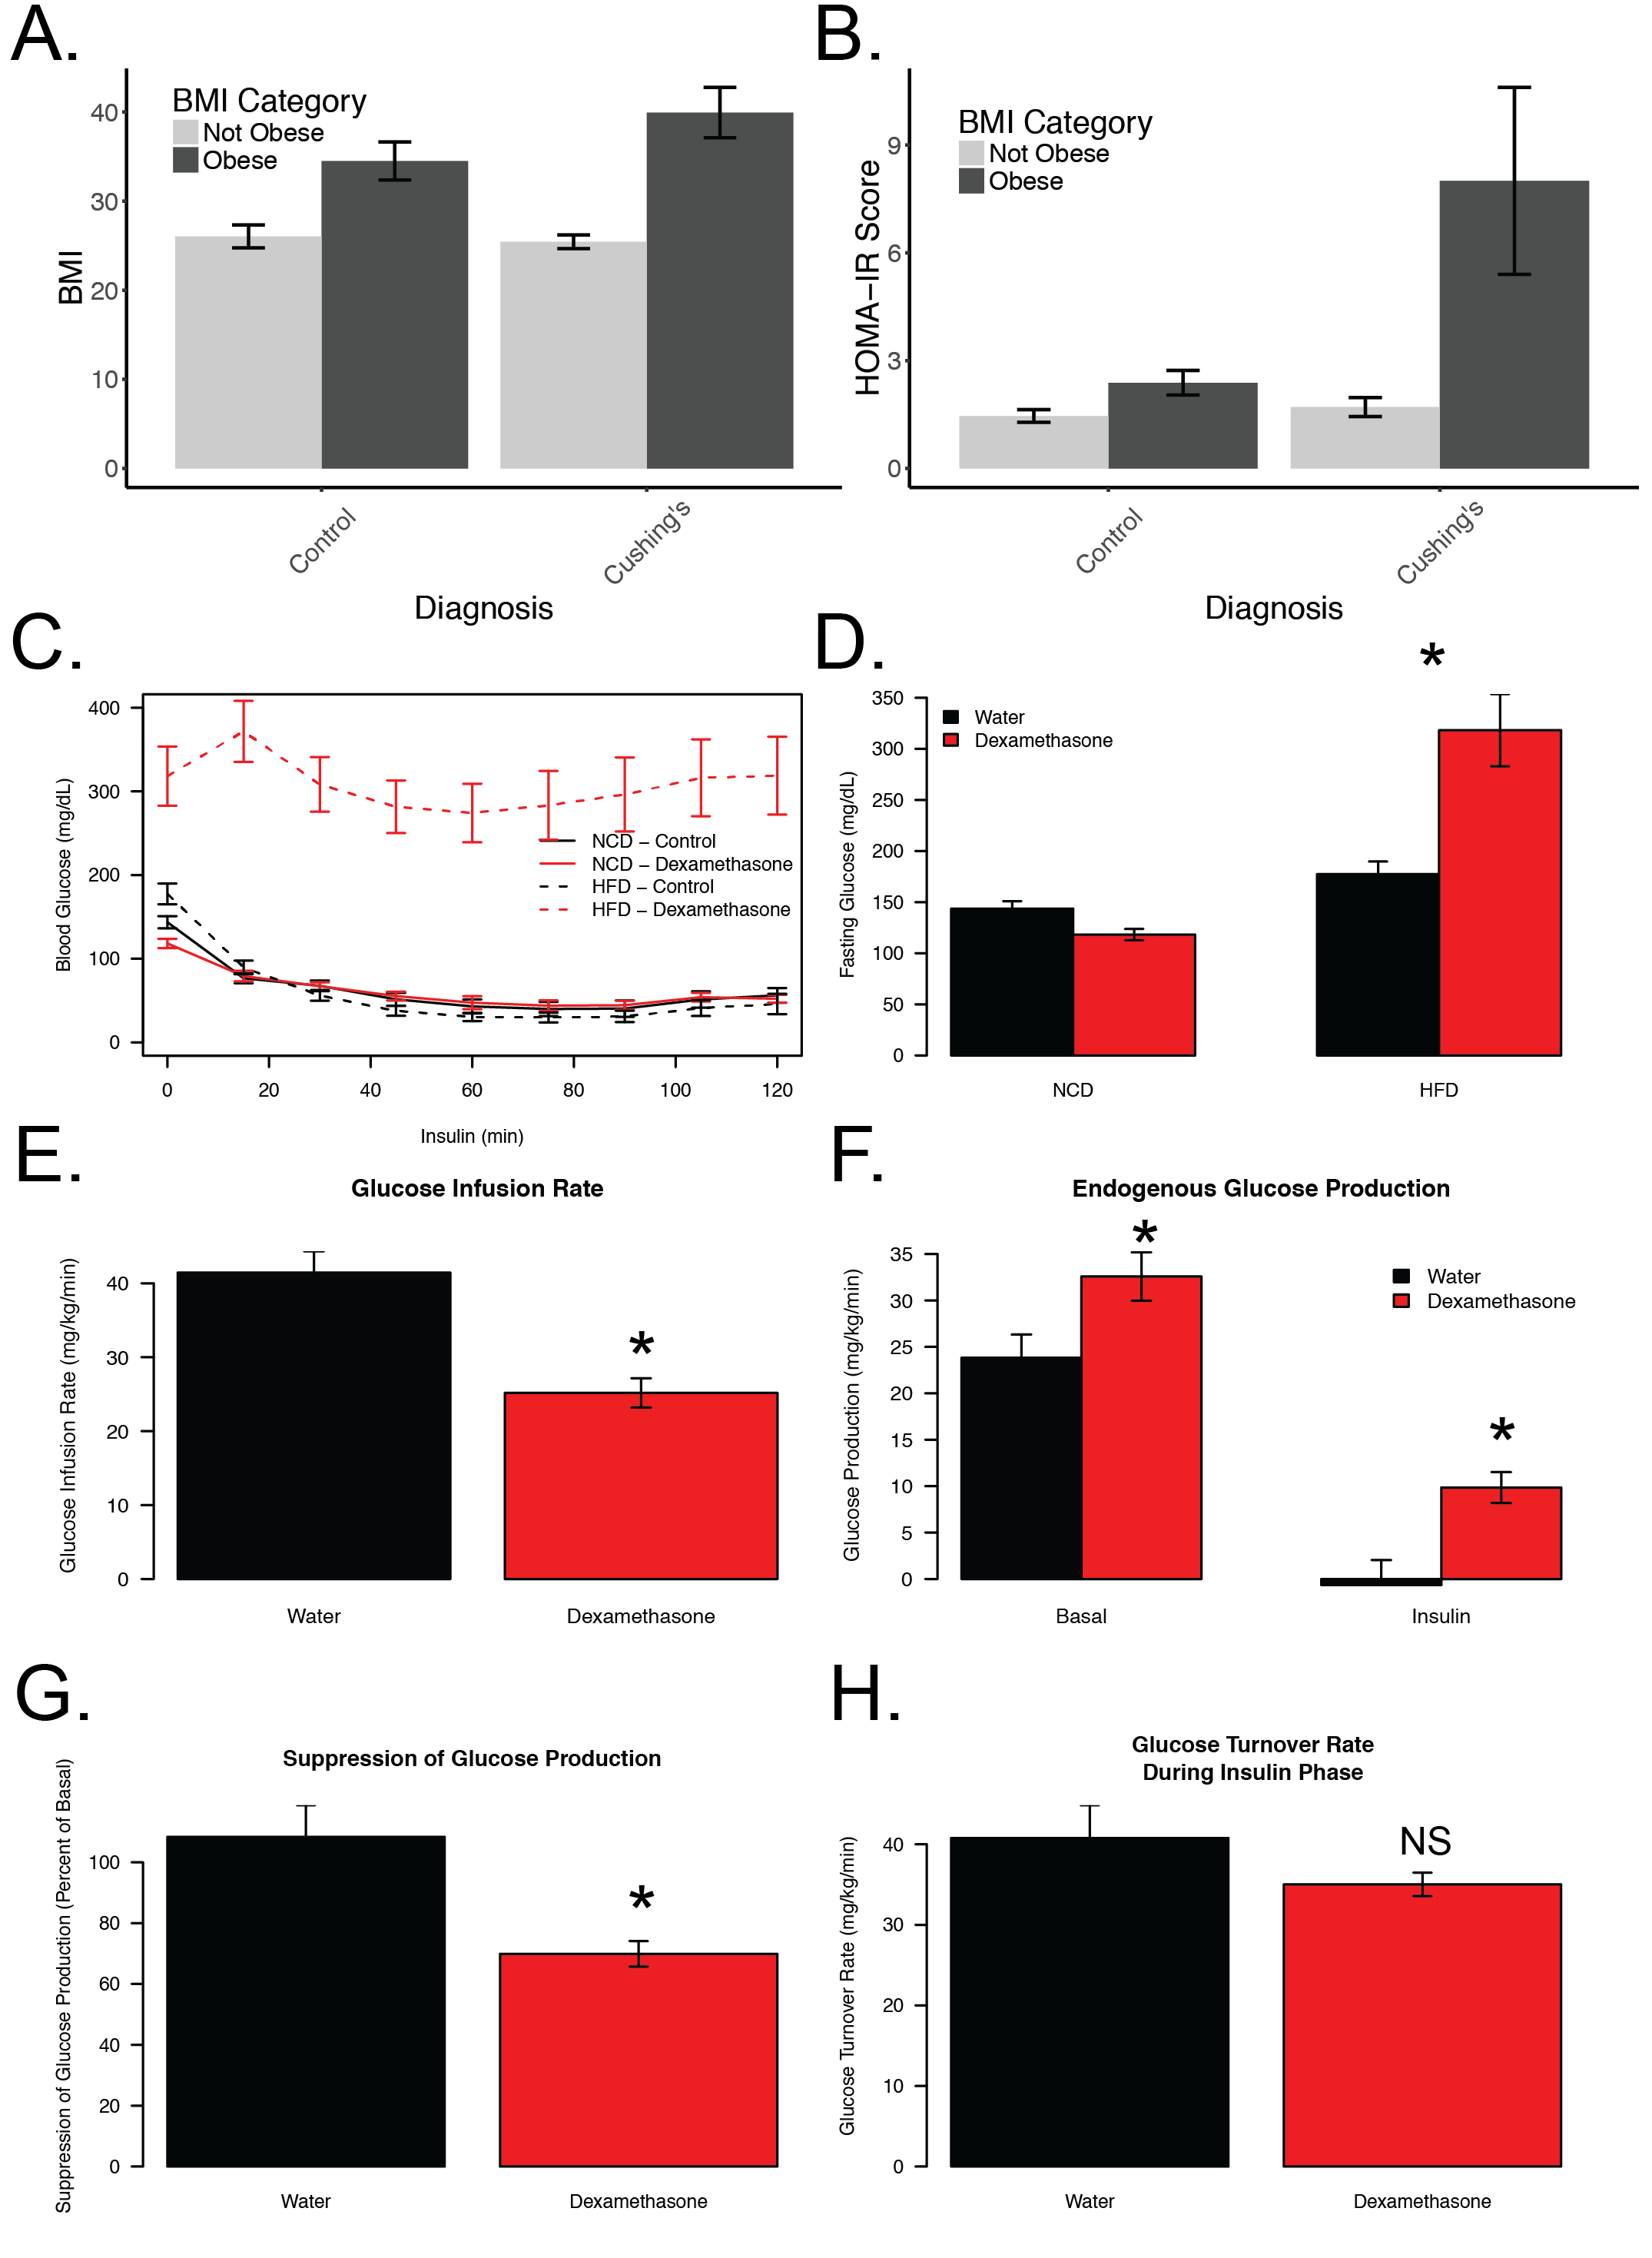
\includegraphics[width=\textwidth]{Figures_Figure_1.png}
  \end{center}
  \caption{\textbf{Reductions in glucose handling are exacerbated in obese individuals with elevated glucocorticoids.}Cushing’s (non-obese n=3; obese n=5) and control (non-obese n=5; obese n=6) BMI (A) and HOMA-IR scores (B) stratified by obesity status. Mouse blood glucose levels during insulin tolerance test (C) and prior to insulin injection (basal; D). Insulin was given via i.p. injection at a concentration of 2.5mU/kg following five weeks of dexamethasone (NCD n=12; HFD n=12) or vehicle (NCD n=12; HFD n=12) treatment and 17 weeks of diet. Mouse glucose infusion rate (GIR; E) and endogenous glucose production (EGP; F) during euglycemic clamp following 3 weeks of dexamethasone (n=14) or vehicle (n=11) treatment and 11 weeks of HFD. For clamp experiments, insulin was infused at 8 mU/kg following a prime continuous infusion of 40mU/kg bolus. All mice were fasted for 5-6 hours prior to experiments. Asterisks in between two bars of the same condition indicate a significant interaction between diet and treatment. Centered asterisks indicated statistically significant treatment effect.}
 \label{fig:1}
\end{figure}

To investigate if obesity status influences insulin sensitivity in the
presence of elevated glucocorticoids we performed an insulin tolerance
test (ITT) on lean (NCD) and diet-induced obese (HFD) mice that were
untreated (Control) or treated with glucocorticoids (Dexamethasone;
Figure 1C). HFD-fed, dexamethasone-treated mice were significantly more
resistant to insulin-stimulated glucose uptake when compared to all
other groups (Figure 1D). Additionally, HFD dexamethasone-treated mice
exhibited dramatic fasting hyperglycemia, with a significant interaction
between diet and drug (p=0.00009; Figure 1E). While HFD animals had a
24\% increase in fasting glucose when compared to NCD animals, in the
presence of Dexamethasone, HFD-fed animals had a 122\% increase in
fasting glucose relative to NCD controls not treated with dexamethasone.
In the lean, NCD-fed animals, dexamethasone caused an 18\% decrease in
fasting glucose.

To evaluate glucose homeostasis in more detail we performed a
hyperinsulinemic-euglycemic clamp in obese mice (11 weeks of HFD)
treated with dexamethasone for the three weeks. This shorter
HFD/dexamethasone exposure still caused dramatic insulin resistance, and
hyperglycemia (Supplementary Figure 1A-B) and reductions in lean mass,
but no differences in fat mass between the groups (Supplementary Figures
1C-D). Animals were clamped while conscious and glucose levels during
the clamp (Supplementary Figure 1E) as well as insulin turnover rate
(Supplementary Figure 1F) were similar between groups. During the
hyperinsulinemic phase, the glucose infusion rate was 39\% lower in
obese dexamethasone-treated mice when compared to obese controls
indicating insulin resistance at euglycemia (Figure 1E). Basal
endogenous glucose production (EGP) was 37\% higher in the
dexamethasone- treated group (p=0.026). Moreover, in the control group,
EGP was reduced to near zero by a high dose of insulin but only reduced
70\% in the dexamethasone group (p=0.0091) resulting in glucose
production being higher during the insulin phase in
dexamethasone-treated mice (p=0.014) when compared to controls (Figure
1F-G). Glucose turnover was slightly decreased in the presence of
insulin (p=0.141; Figure 1H). In spite of these modest changes in
glucose turnover, there were significant reductions in the obese,
dexamethasone-treated animals in 2-deoxyglucose uptake in heart (34\%
reduced, p=0.0003) and gastrocnemius tissues (68\% reduced; p=0.00002;
Supplementary Figures 1G-H). These data suggest that increased glucose
production and impaired suppression by insulin are the primary causes of
insulin resistance and hyperglycemia in obese, dexamethasone-treated
animals.

\subsection*{HFD-Induced Liver Steatosis in Dexamethasone-Treated
mice}\label{hfd-induced-liver-steatosis-in-dexamethasone-treated-mice}

Obesity and chronic elevations in glucocorticoids are associated with
increased liver fat and NAFLD (13,2). We observe increases in plasma
ALT, a liver enzyme associated with liver disease, in obese Cushing's
patients (38\% increase in non-obese subjects versus a 2.8 fold increase
in obese subjects, p=0.13 for the interaction of disease and obesity
status; Figure 2A). In our mouse model of HFD-fed, dexamethasone-treated
mice, we observe drastically elevated liver triglycerides when compared
to all other groups with a significant interaction of drug and diet
(p=0.000068; Figure 2B). In support of this, H\&E staining of hepatic
tissue clearly depicts exacerbated lipid levels in the obese,
glucocorticoid-treated group when compared to HFD-fed or
dexamethasone-treated controls (Figure 2C).

\begin{figure}
  \begin{center}
    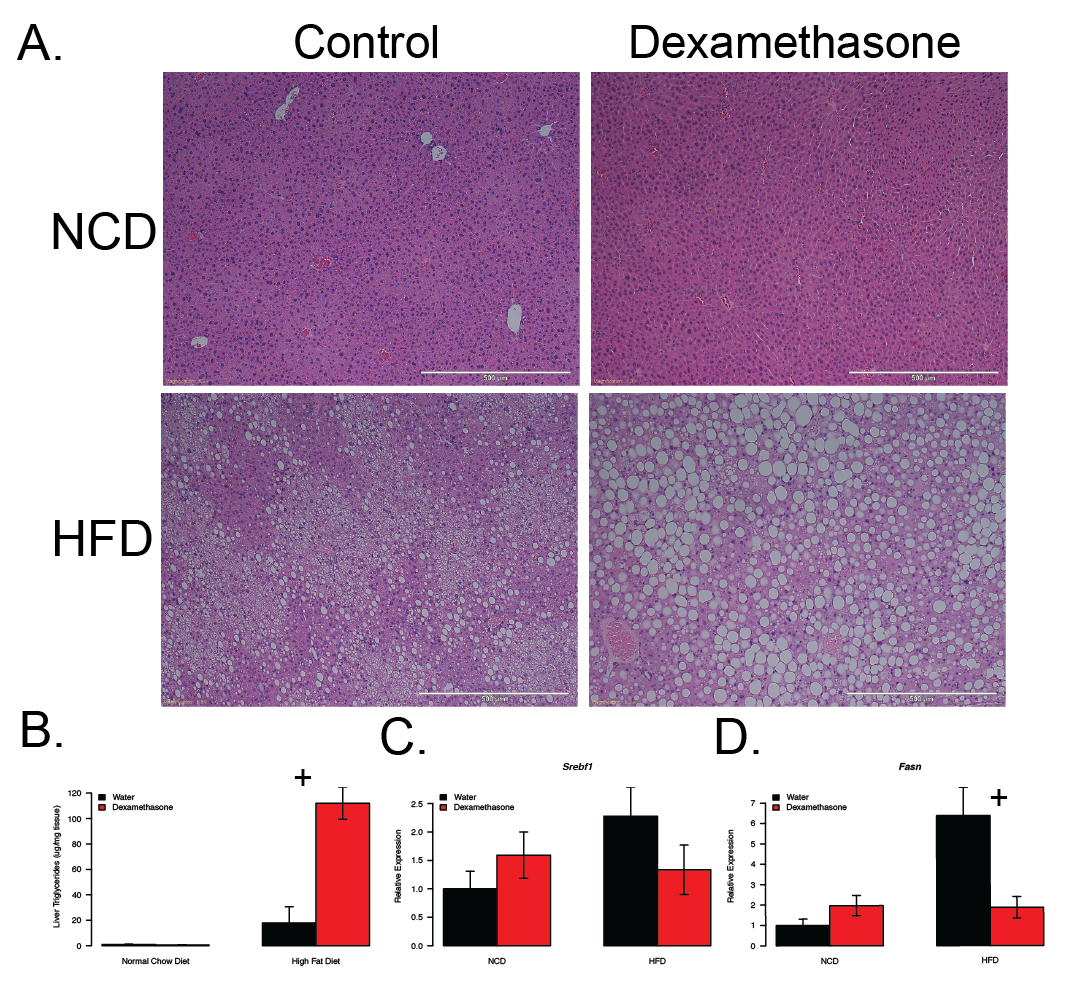
\includegraphics[width=\textwidth]{Figures_Figure_2.png}
  \end{center}
  \caption{\textbf{Increased glucocorticoids lead to greater severity of hepatic steatosis in obese mice.}
Patient ALT levels (A). Mouse hepatic triglyceride levels (B) and Hematoxylin and Eosin stained liver sections (C) and qPCR of hepatic de novo lipogenic transcripts (D, E). Mice were euthanized at 28 weeks of age following six weeks of dexamethasone (NCD n=7; HFD n=5) or vehicle (NCD n=6; HFD n=9) treatment and 18 weeks of diet. Liver stains are representative samples from each group. Asterisks indicate a significant interaction between diet and treatment.}
 \label{fig:2}
\end{figure}

We used qPCR to measure the expression of genes involved in hepatic
\emph{de novo} lipogenesis, \emph{Srebf1} and \emph{Fasn}, in liver
lysates (Figure 2D). We observed a significant effect of diet and drug
on \emph{Fasn} expression (p=0.014), and although both transcripts were
somewhat elevated in response to HFD alone, no synergism in expression
levels was observed with dexamethasone. This finding indicates that
lipid accumulation in response to dexamethasone treatment is likely
occurring via mechanisms other than accelerated glucocorticoid-dependent
activation of \emph{de novo} lipogenesis.

\subsection*{Dexamethasone Causes Decreased Fat Mass in HFD-Fed
Mice}\label{dexamethasone-causes-decreased-fat-mass-in-hfd-fed-mice}

To understand the how dexamethasone effects body composition in these
animals, we measured fat mass via EchoMRI. We observed reductions in fat
mass in the HFD-fed dexamethasone-treated group (Figure 3A-B). These
reductions do not appear to be depot-specific, as we observe reductions
in both iWAT (65\% reduced) and eWAT mass (59\% reduced) at the end of
the study in the HFD-fed animals treated with dexamethasone (Figure 3C).
There were no significant reductions in fat mass, either by MRI or gross
tissue weights of iWAT or eWAT depots in response to dexamethasone
treatment in the chow-fed groups (Figure 3B-C). To determine if changes
in body composition could be explained by changes in food consumption
throughout this study (Figure 3D), we compared food intake between the
groups. Surprisingly, we found that the dexamethasone-treated HFD
animals ate slightly more food, even though they lost substantial fat
mass throughout the study (11\% increase, p=0.032). These data suggest
that the weight loss in obese animals provided dexamethasone is not due
to reductions in food intake.

\begin{figure}
  \begin{center}
    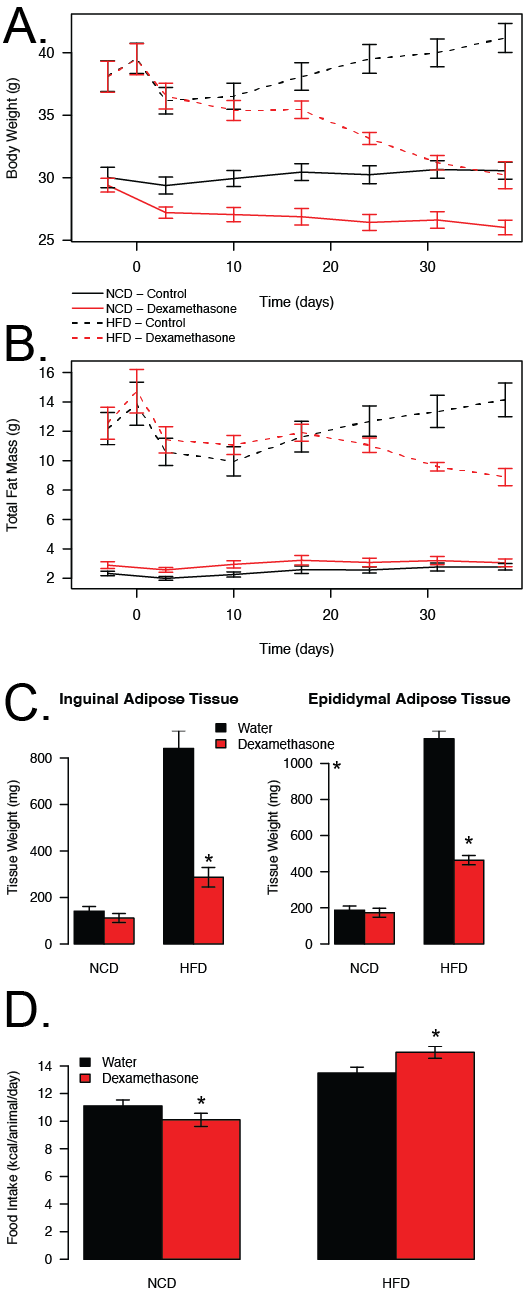
\includegraphics[width=0.5\textwidth]{Figures_Figure_3.png}
  \end{center}
  \caption{\textbf{Dexamethasone treatment reduces fat mass in obese mice.}  Weekly total body mass (A) and fat mass (B) measures via EchoMRI in mice over the course of treatment (solid lines represent NCD mice and dashed lines represent HFD mice). Adipose tissue weights in 16 hour fasted mice following euthanasia (C). Mice were euthanized at 28 weeks of age following six weeks of dexamethasone (NCD n=8; HFD n=12) or vehicle (NCD n=8; HFD n=22) treatment and 18 weeks of diet. Food consumption measured weekly over the course of treatment (D). Asterisks indicate a statistically significant treatment effect.
}
 \label{fig:3}
\end{figure}

\subsection*{Dexamethasone Treatment Results in Increased Lipolysis}

One potential mechanism that could explain reduced adiposity, increased
insulin resistance and NAFLD is accelerated adipocyte lipolysis.
Lipolysis has previously been associated with insulin resistance
(25,31), is known to be elevated in patients with NAFLD(28), and has
been shown to increase with glucocorticoid treatment (18,22--24). To
assess whether dexamethasone was directly affecting the lipid content in
adipose tissue, we measured markers of adipocyte lipolysis in cultured
adipocytes. 3T3-L1 fibroblasts were undifferentiated (pre-adipocytes),
differentiated and treated with vehicle (mature adipocytes) or
dexamethasone following differentiation (mature adipocytes
+dexamethasone) over a 15-day period. Dexamethasone treatment following
differentiation led to decreased lipid content (52.4\% reduction,
p=0.005) and a 71\% increase in the amount of glycerol in the media
(p=0.001), suggesting increased lipolysis (Figure 4B). In order to
identify a potential GR-dependent lipolytic target, we evaluated the
levels of ATGL, the rate limiting enzyme in lipolysis. Expression of
ATGL (encoded by the \emph{Pnpla2} gene) was enhanced following
dexamethasone treatment in 3T3-L1 cells at both the transcript (2.7
fold, p=0.002; Figure 4C) and protein (4.2 fold, p=0.025; Figure 4D-E)
levels. These data show that glucocorticoids elevate both ATGL levels
and metabolites of lipolysis in cultured adipocytes.

\begin{figure}
  \begin{center}
    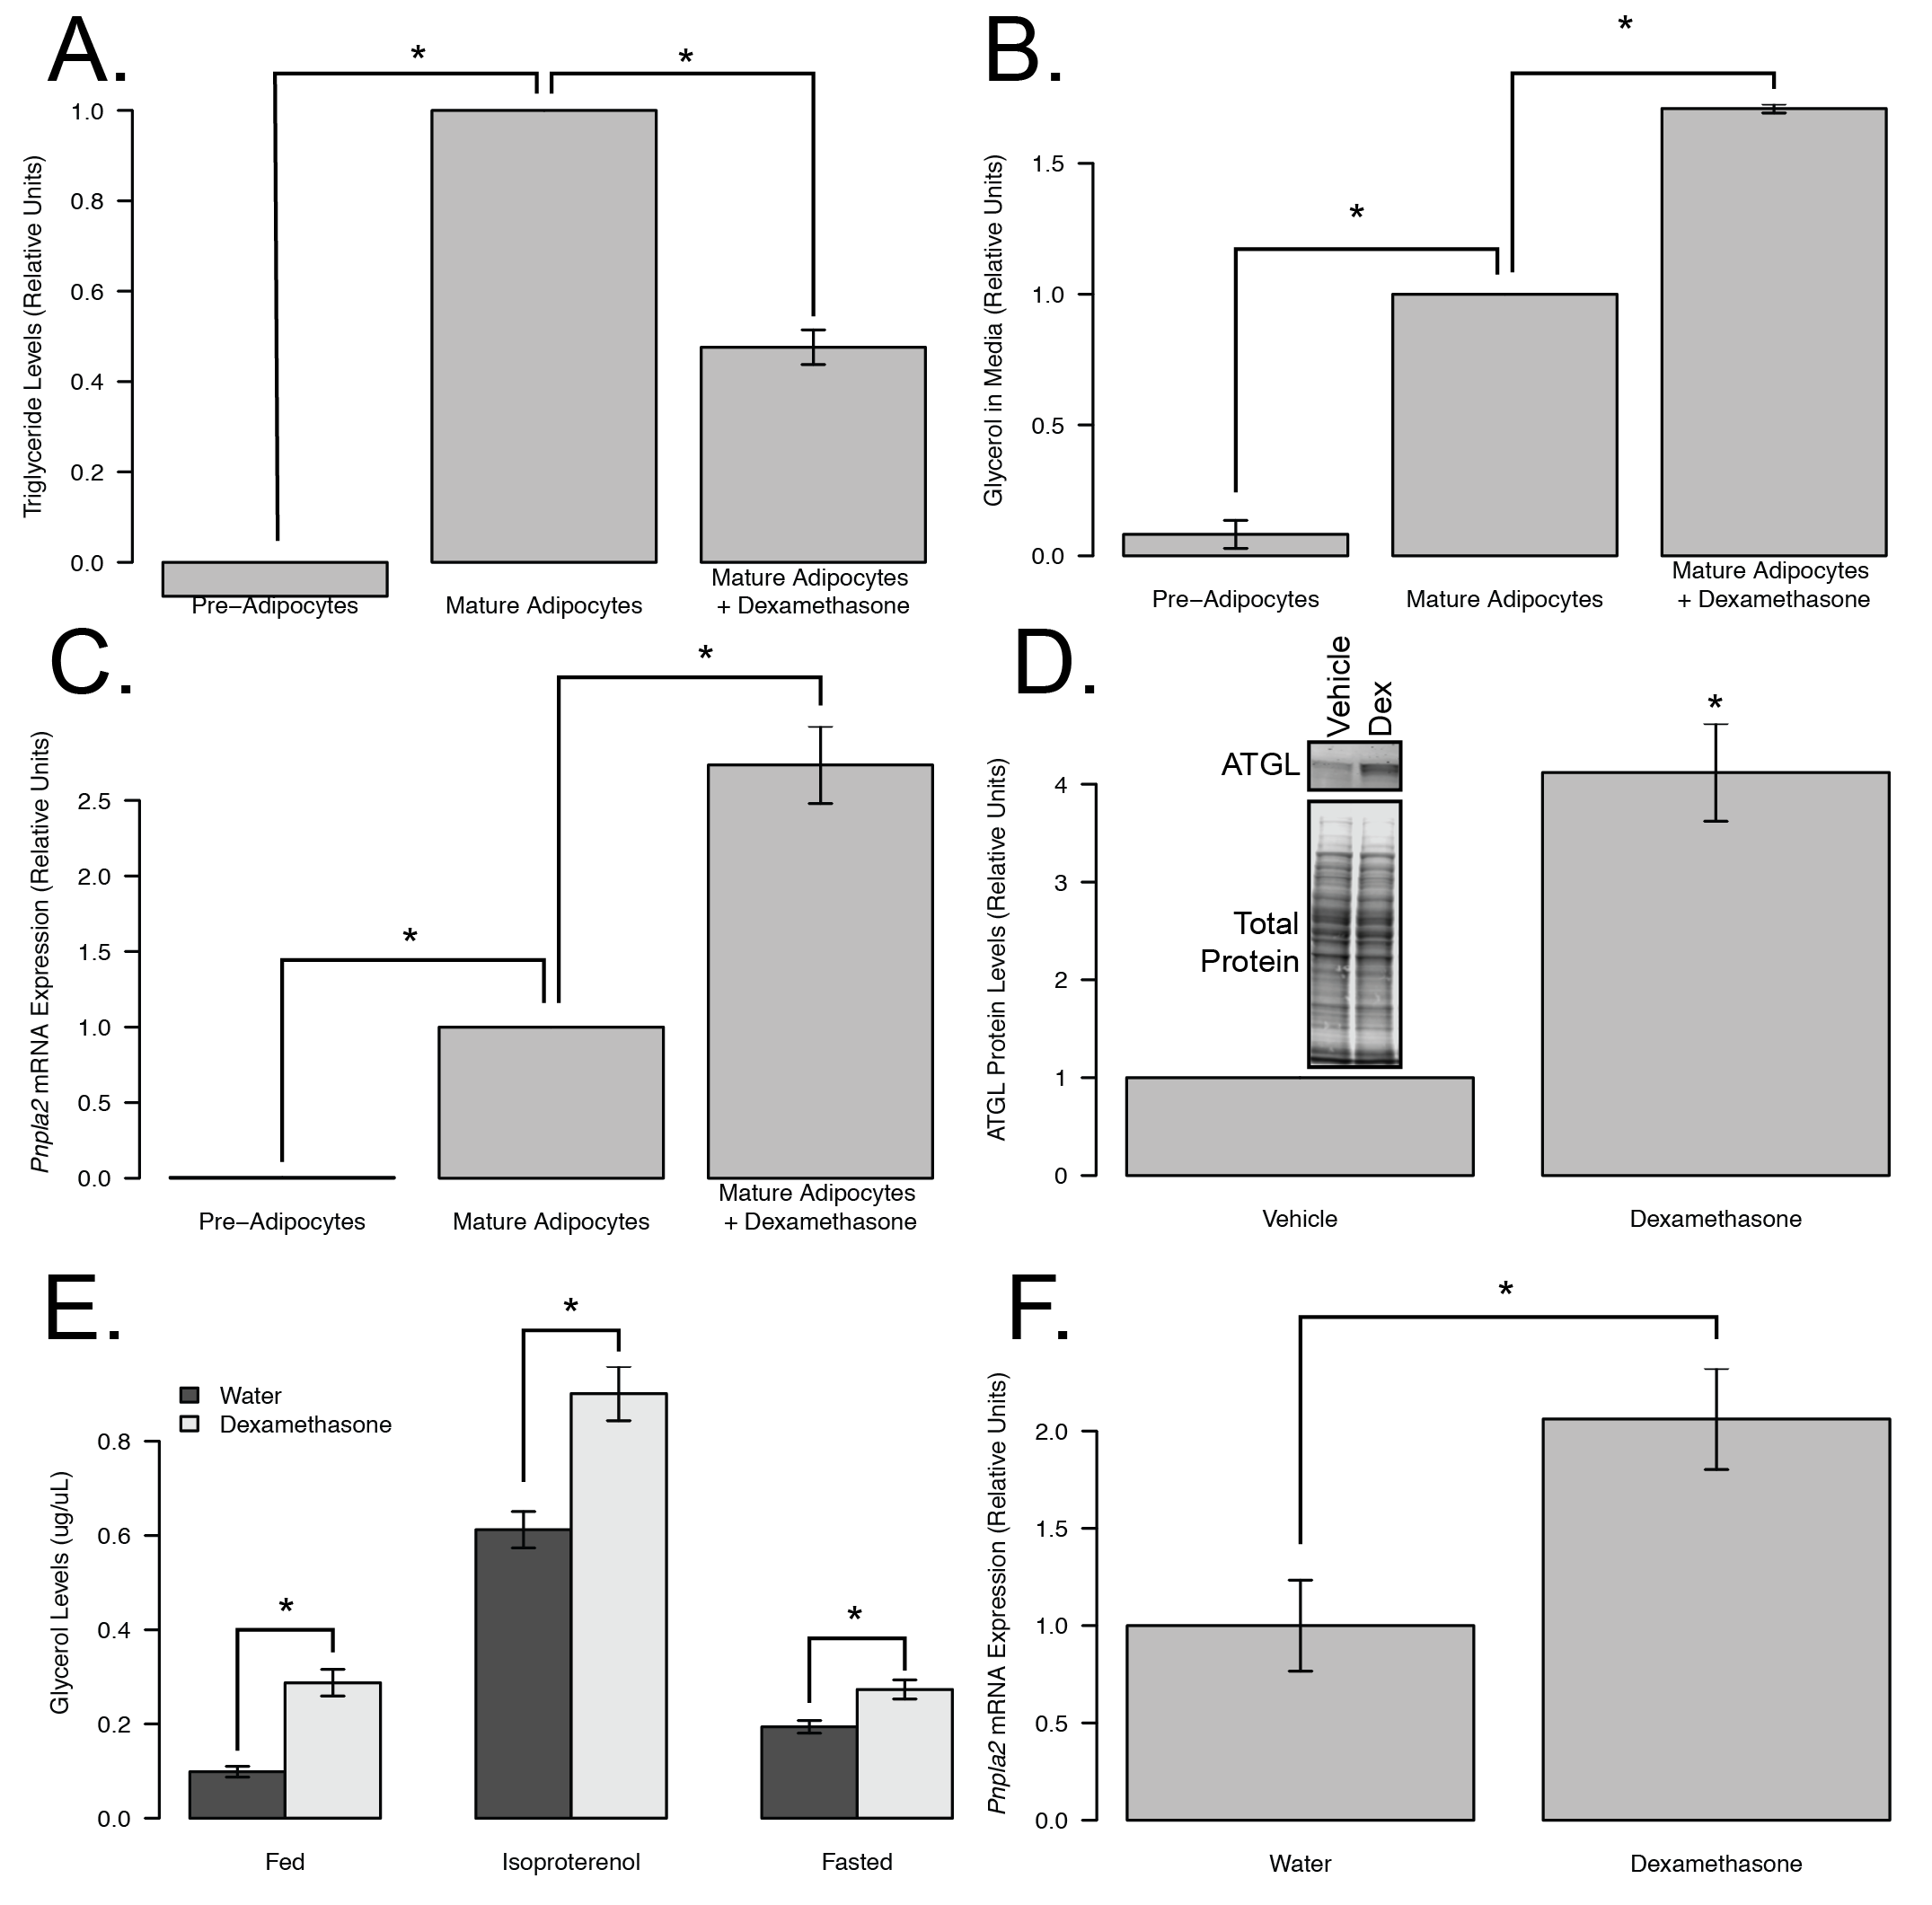
\includegraphics[width=\textwidth]{Figures_Figure_4.png}
  \end{center}
  \caption{\textbf{ Dexamethasone treatment induces lipolysis in vivo and in vitro.}  Triglyceride levels (A), glycerol released in media (B), qPCR of lipolytic transcripts (C), and western blot of ATGL (D) from non-differentiated (pre-adipocytes; n=2) or differentiated 3T3-L1 mouse adipocytes (mature adipocytes) following five days of dexamethasone (n=3) or vehicle treatment (n=3). Serum fatty acid and glycerol levels at basal (fed) and following stimulation (10mg/kg isoproterenol or 16hr fast; E) and qPCR of IWAT lipolytic transcripts (F) in 22-week-old, 12-week dexamethasone- (basal and isoproterenol n=7; fasted serum and qPCR n=4) or vehicle- (basal and isoproterenol n=12; fasted serum and qPCR n=11) treated, chow-fed mice with the exception of isoproterenol-stimulated glycerol, which was performed one week prior to euthanasia. Asterisks indicated statistically significant treatment effect.}
 \label{fig:4}
\end{figure}

To assess the effects of glucocorticoid-induced lipolysis \emph{in
vivo,} we determined glycerol levels in animals chronically exposed to
glucocorticoids in basal and stimulated conditions (Figure 4E).
Stimulation of lipolysis was achieved via isoproterenol, a $\beta$-adrenergic
receptor agonist, or by a 16-hour fast. Twelve weeks of dexamethasone
treatment led to significant increases in glycerol in the fed (2.9
fold), fasted (1.5 fold) and isoproterenol-stimulated (1.4 fold, all
groups p\textless{}0.05) conditions, indicating that dexamethasone
enhances basal and stimulated lipolysis \emph{in vivo} in chow-fed mice,
as has been previously reported (45). Consistent with these findings,
mRNA analysis from iWAT of these mice showed an upregulation of
\emph{Pnpla2} transcripts in the dexamethasone-treated mice compared to
controls (2.1 fold, p=0.016; Figure 4F).

Since the HFD-fed, dexamethasone-treated mice have more severe insulin
resistance and hepatic lipid accumulation than the chow fed mice, we
quantified serum glycerol concentrations following a 16-hour fast
(Figure 5A) as a surrogate measure of lipolysis. We observed a nearly
two-fold increase in serum glycerol levels by 6 weeks of dexamethasone
treatment in the HFD-fed animals, compared with only a 18\% increase in
chow-fed mice. There was a significant interaction between dexamethasone
exposure and diet (p=0.017) on glycerol levels. We then asked if the
increase in lipolytic metabolites was suppressed by insulin during the
hyperinsulinemic euglycemic clamp in the obese mice (Figure 5B).
Consistent with our previous results, there was a 40\% elevation in
serum basal non-esterified fatty acids (NEFA's) in response to 3 weeks
of dexamethasone treatment (p=0.004). During the insulin phase,
dexamethasone treatment attenuated the ability of insulin to suppress
serum NEFA levels by with insulin leading to a 71\% reduction in water
controls compared to only a 48\% reduction in dexamethasone-treated mice
(p=0.058). These findings suggest that dexamethasone elevates lipolysis
in the obese setting and likely attenuates the suppressive effects of
insulin.

\begin{figure}
  \begin{center}
    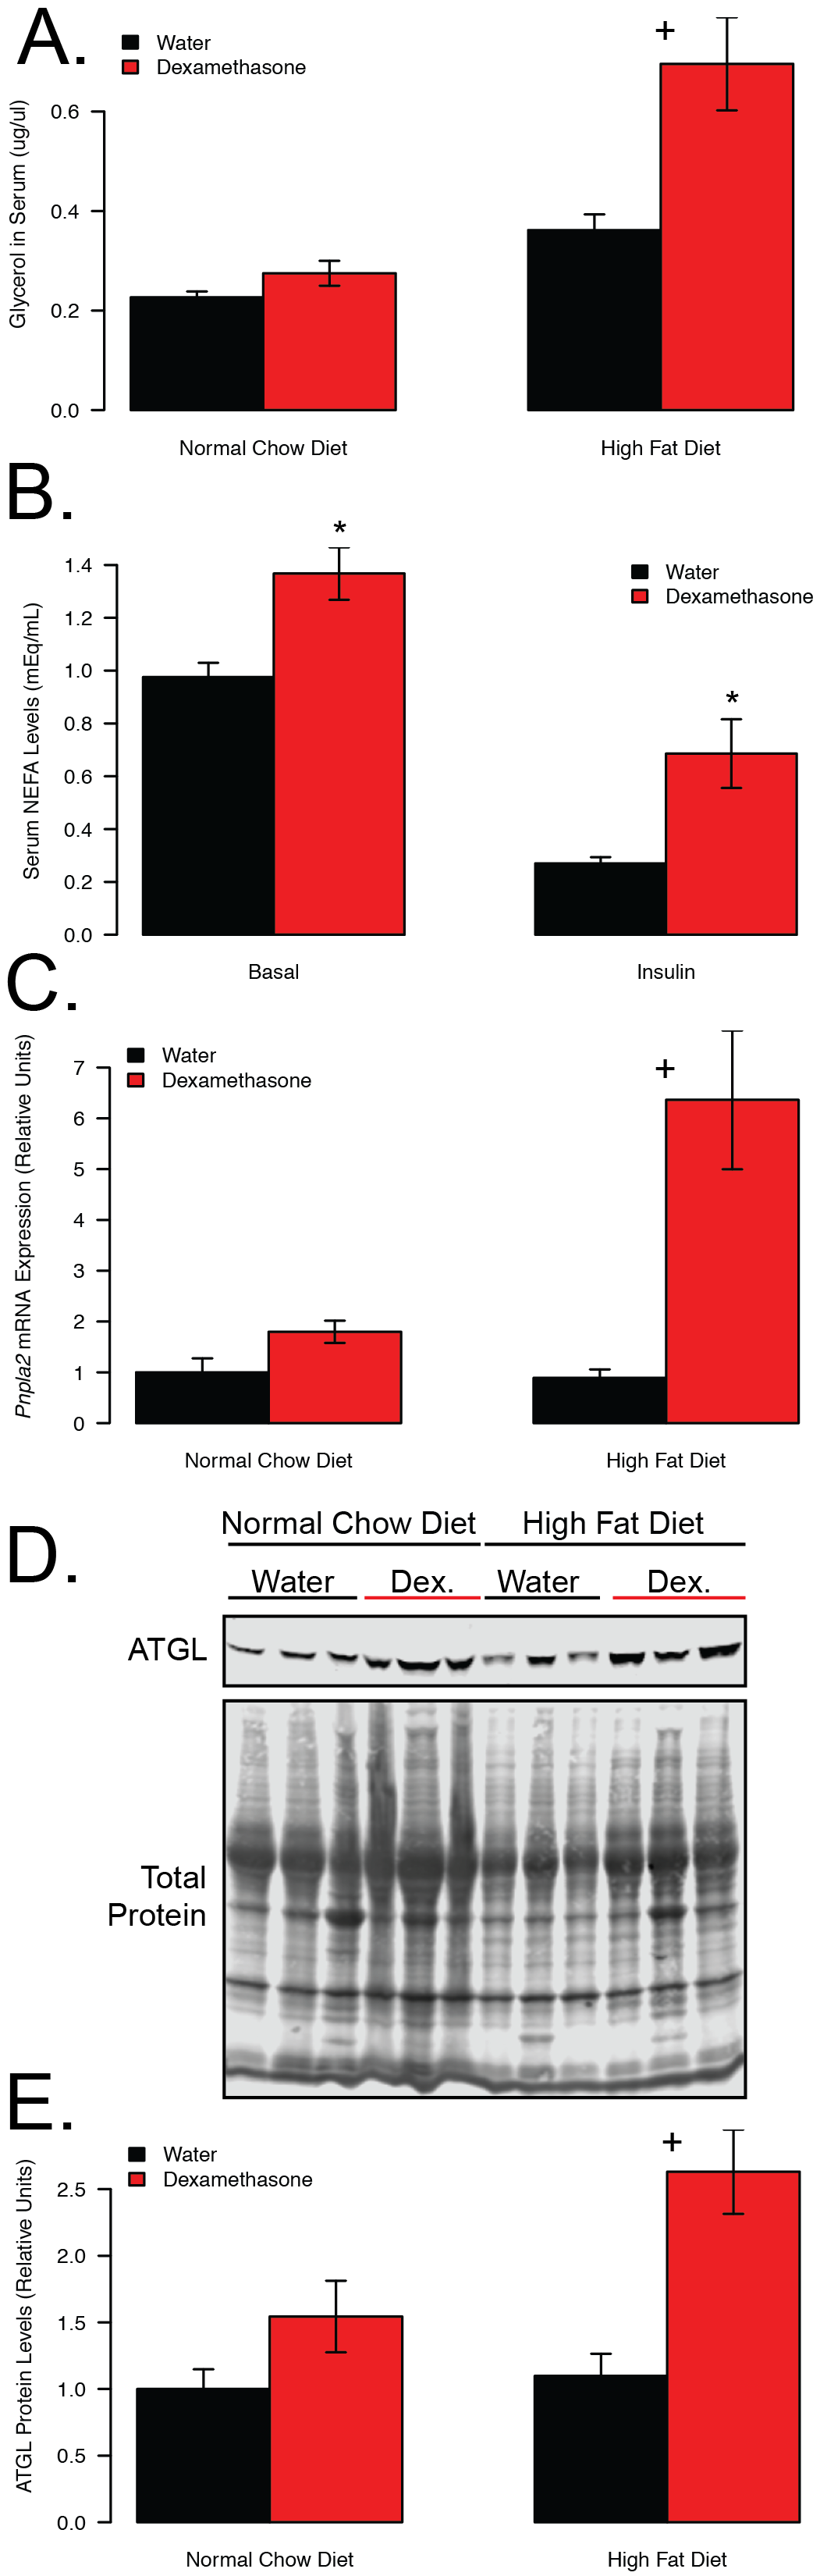
\includegraphics[width=0.35\textwidth]{Figures_Figure_5.png}
  \end{center}
  \caption{\textbf{Obesity exacerbates dexamethasone-induced lipolysis.}  Serum glycerol (A) following 16 hour fast, serum NEFA in obese dexamethasone treated (n=14) or control (n=11) mice following a 5 hour fast, before and after insulin during hyperinsulinemic euglycemic clamp (B), qPCR of Pnpla2 transcripts from iWAT (C), and western blot image (D) and quantification (E) of ATGL protein from iWAT. Mice from A, C, D and E were euthanized at 28 weeks of age following six weeks of dexamethasone (NCD n=8; HFD n=10) or vehicle (NCD n=8; HFD n=10) treatment. Asterisks in between two bars of the same condition indicate a significant interaction between diet and treatment. Centered asterisks indicated statistically significant treatment effect.}
 \label{fig:5}
\end{figure}

We quantified mRNA and protein expression of the lipolytic enzyme ATGL,
in the iWAT of these mice (5C-E). Consistent with the hypothesis that
ATGL activation could drive increased lipolysis in HFD and
dexamethasone-treated mice, expression of ATGL was elevated in both
dexamethasone-treated groups, with a significant synergistic effect of
glucocorticoids and obesity at both the transcript (p=0.02 for the
interaction) and protein (p=0.043 for the interaction) levels. These
data support the hypothesis that glucocorticoid-stimulated lipolysis is
augmented in the context of obesity, potentially via increased
transactivation of \emph{Pnpla2}/ATGL.

\section*{Discussion}

Chronic glucocorticoid elevations are associated with many
co-morbidities such as increased fat mass (18,20,21), decreased muscle
mass (17--19), insulin resistance (4,5) and NAFLD (2,3). These adverse
effects are similar to those seen in obesity; however, the combination
of chronically elevated glucocorticoids in the context of pre-existing
obesity has not been assessed. Here, we show that the effects of
glucocorticoid-induced insulin resistance and NAFLD are exacerbated when
paired with obesity.

We found that obese patients with Cushing's disease have higher waist
circumference (data not shown), indicative of central adiposity, and
have a tendency for increases in HOMA-IR score, suggesting increased
insulin resistance. Additionally, we observed increases in the liver
enzyme ALT, a marker of liver disease. In line with these findings,
increases in central adiposity, as is frequently observed in people with
obesity, has been associated with enhanced fatty acid flux (i.e.
lipolysis) when compared to lower body fat stores (46), which is thought
to contribute to insulin resistance and fatty liver (25,47).

There are two limitations to these interpretations: one is the small
sample size, and two, that it is not possible to determine the
physiological status of Cushing's patients before they develop a tumor;
therefore, we could not discern whether obesity was present prior to or
after development of Cushing's disease. To address the question of
whether the obese state modulates the effects of glucocorticoid excess,
we designed mouse studies that assess the metabolic outcomes frequently
associated with both obesity and exposure to elevated glucocorticoid
concentrations.

We found that HFD-fed, dexamethasone-treated mice exhibited
hyperglycemia and severe insulin resistance. This was primarily due to
increased endogenous glucose production in these animals. HFD and
dexamethasone also led to significant elevations in liver fat,
consistent with a trend towards elevated ALT levels seen in the obese
Cushing's patients. Cushing's disease is often paired with increased fat
mass, which has been proposed to contribute to fatty liver (48,49).
Indeed, obesity is a known risk factor of NAFLD (13,14). Previous work
from our lab shows increased fat mass, following 12 weeks of
dexamethasone treatment (18) in chow-fed mice, in accordance with what
others have reported (50). However, to our surprise, the glucocorticoid
treatment in obese mice led to an overall reduction in adiposity.
Therefore, when comparing HFD control mice to HFD dexamethasone-treated
mice, increased fat mass is not the major mechanism behind the observed
exacerbations in insulin resistance and increased liver fat.

Lipolysis has been linked to increased gluconeogenesis by several
studies (51--54). One potential mechanism is that the increased flux of
fatty acids, oxidized in the liver to acetyl-CoA, activate pyruvate
carboxylase and gluconeogenesis (53,54). Glucocorticoids are known to
stimulate lipolysis (18,22--24), possibly as a way to promote
gluconeogenesis to maintain blood glucose levels, a key function of
these hormones. Lipolysis has been implicated in insulin resistance
(25,31) and NAFLD (28) and there is evidence that it is enhanced in the
obese state (55). We found synergistic elevations in glycerol,
indicative of enhanced lipolysis, as well as in hepatic fat accumulation
in the HFD-fed dexamethasone-treated mice, but no data supporting
enhanced hepatic \emph{de novo} lipogenesis. These findings suggest that
lipolysis may drive enhanced hepatic lipid accumulation in these mice.

There is some debate as to which genes glucocorticoids are acting on to
promote lipolysis. Downregulation of \emph{Pde3b} (56) and upregulation
of -adrenergic receptors (57) and ATGL transcripts (35,58,59) have been
proposed as possible mechanisms. We assessed all of the previously
proposed targets and found ATGL, the rate limiting enzyme for adipose
triglyceride lipolysis, to be synergistically activated by obesity and
glucocorticoid-treatment. These findings bear a resemblance to
elevations in glycerol levels in obese, dexamethasone-treated mice when
compared to diet or glucocorticoids alone. The mechanisms by which
obesity and glucocorticoids synergize to activate ATGL expression are
not clear at this time, nor are the relative contributions of other
glucocorticoid receptor-dependent targets.

Further research is needed to determine whether the insulin resistance
observed is due to obesity or the high fat content of the diet. We
evaluated glucocorticoid treatment in obesity; however, Riddell and
colleagues have reported similar findings when giving HFD and
glucocorticoids in concert to rats, prior to the onset of obesity
(15,16,60). Further studies are needed to determine whether diet or
obesity status or both are the source of this elevated metabolic risk to
glucocorticoids, and whether these mechanisms are similar.

In summary, glucocorticoids are commonly prescribed drugs used to treat
a multitude of health issues, but are known to induce a variety of
adverse metabolic effects. Their actions in persons with obesity are not
yet clear, even though there are a huge number of obese individuals
routinely taking prescription glucocorticoids. The data presented here
show that the obese state exacerbates several co-morbidities associated
with chronically elevated glucocorticoids. These effects should be
considered by physicians when determining glucocorticoid treatment
options for patients with obesity. Future studies will determine whether
blocking glucocorticoid/lipolytic action in the fat tissue is beneficial
for preventing or enhancing recovery from glucocorticoid-induced
metabolic disturbances.

\section*{Acknowledgements}\label{acknowledgements}

This study was supported by funds from NIH Grant R01-DK107535 (DB). This
study also utilized the University of Michigan Metabolism, Bariatric
Surgery and Behavior Core (U2C-DK110768), the Michigan Nutrition Obesity
Research Center (P30-DK089503) and the University of Michigan
Comprehensive Cancer Center Core (P30-CA062203). Erin Stephenson is
partially supported by funding from Le Bonheur Children's Hospital, the
Children's Foundation Research Institute and the Le Bonheur Associate
Board . We would like to thank Jennifer DelProposto and Carey Lumeng for
assistance with imaging liver sections, and Melanie Schmitt for
assistance with glucose clamp studies. We would like to thank the other
members of the Bridges laboratory, Thurl Harris (University of Virginia)
and Edwards Park (UTHSC) for insights on this work.

\section*{Author Contributions}
D. Bridges acquired funding. D. Bridges, I. Harvey and I. Hochberg were responsible for conceptualizing the study. D. Bridges, I. Harvey and N. Qi designed the experiments. I. Harvey performed all cell experiments. I. Harvey, E. Stephenson and J. Redd performed mouse experiments. D. Bridges and Q. Tran performed statistical analyses. I. Harvey wrote the manuscript. I Harvey and D. Bridges edited and reviewed the manuscript. All authors were involved in discussions. This manuscript has been approved by all authors.

\section*{References}\label{references}

1. Rutters F, Nieuwenhuizen AG, Lemmens SGT, Born JM,
Westerterp-plantenga MS. Hypothalamic -- Pituitary -- Adrenal ( HPA )
axis functioning in relation to body fat distribution. 2010;738--43.

2. Rockall A, Sohaib S, Evans D, Kaltsas G, Isidori A, Monson J, Besser
G, Grossman A, Reznek R. Hepatic steatosis in Cushing's syndrome: a
radiological assessment using computed tomography. Eur J Endocrinol
{[}Internet{]}. 2003;149:543--8. Available from:
http://www.eje-online.org/cgi/doi/10.1530/eje.0.1490543

3. Cerda J, Fardella CE, Arrese M. Overexpression of 11 b
-hydroxysteroid dehydrogenase type 1 in visceral adipose tissue and
portal hypercortisolism in non-alcoholic fatty liver disease.
2012;392--9.

4. Pivonello R, Martino MC De, Leo M De, Lombardi G, Colao A. Cushing's
Syndrome. 2008;37:135--49.

5. Resmini E, Minuto F, Colao A, Ferone D. Secondary diabetes
associated with principal endocrinopathies: the impact of new treatment
modalities. 2009;85--95.

6. Overman R a., Yeh JY, Deal CL. Prevalence of oral glucocorticoid
usage in the United States: A general population perspective. Arthritis
Care Res. 2013;65:294--8.

7. Fardet L, Petersen I, Nazareth I. Original article Prevalence of
long-term oral glucocorticoid prescriptions in the UK over the past 20
years. 2011;

8. Hsiao C, Ph D, Cherry DK, Beatty PC, Ph D, Rechtsteiner EA, Care H.
National Ambulatory Medical Care Survey: 2007 Summary. 2010;

9. Laugesen K, Otto J, Jrgensen L, Srensen HT, Petersen I. Systemic
glucocorticoid use in Denmark: a population-based prevalence study.
2017;1--6.

10. Karam JH, Grodsky GM, Ph D, Forsham PH. Excessive Insulin Response
to Glucose in Obese Subjects as Measured by Immunochemical Assay.

11. Bagdadea JD, Bierman EL, Porte D, Ii JR, Nih W, Presented GF-. The
Significance of Basal Insulin Levels in the Evaluation of the Insulin
Response to Glucose in Diabetic and Nondiabetic Subjects *. 1967;46.

12. Steffensen C, Pereira AM, Dekkers OM. Prevalence of hypercortisolism
in type 2 diabetes patients: a systematic review and. 2016;

13. Wanless I, Lentz J. Fatty Liver Hepatitis ( Steatohepatitis ) and
Obesity: An Autopsy Study with Analysis of Risk Factors. Hepatology.
1990;12:1106--10.

14. Youssef WI, Mccullough AJ. Steatohepatitis in obese individuals.
2002;16:733--47.

15. Beaudry JL, Anna MD, Teich T, Tsushima R, Riddell MC. Exogenous
Glucocorticoids and a High-Fat Diet Cause Severe Hyperglycemia and
Hyperinsulinemia and Sprague-Dawley Rats. 2013;154:3197--208.

16. Shpilberg Y, Beaudry JL, Souza AD, Campbell JE, Peckett A, Riddell
MC. A rodent model of rapid-onset diabetes induced by glucocorticoids
and high-fat feeding. 2012;680:671--80.

17. Dardevet D, Somet C, Taillandier D, Savary I, Attaix D, Grizard J.
Sensitivity and Protein Turnover Response to Glucocorticoids Are
Different in Skeletal Muscle from Adult and Old Rats Lack of Regulation
of the Ubiquitin-Proteasome Proteolytic Pathway in Aging. J Clin Invest.
1995;96:2113--9.

18. Hochberg I, Harvey I, Tran QT, Stephenson EJ, Barkan AL, Saltiel AR,
Chandler WF, Bridges D. Gene expression changes in subcutaneous adipose
tissue due to Cushing's disease. J Mol Endocrinol {[}Internet{]}.
2015;55:81--94. Available from:
http://www.ncbi.nlm.nih.gov/pubmed/26150553

19. Schakman O, Kalista S, Barb C, Loumaye A, Thissen JP.
Glucocorticoid-induced skeletal muscle atrophy . Int J Biochem Cell
Biol {[}Internet{]}. Elsevier Ltd; 2013;45:2163--72. Available from:
http://dx.doi.org/10.1016/j.biocel.2013.05.036

20. Abad V, Chrousos GP, Reynolds JC, Nieman LK, Hill SC, Weinstein RS,
Leong GM. Glucocorticoid Excess During Adolescence Leads to a Major
Persistent Deficit in Bone Mass and an Increase in Central Body Fat.
2001;16:1879--85.

21. Geer EB, Shen W, Gallagher D, Punyanitya M, Looker HC, Post KD,
Freda PU. Female Patients with Cushing ' s Disease. 2011;73:469--75.

22. Djurhuus CB, Gravholt CH, Nielsen S, Pedersen SB, Mller N, Schmitz
O. Additive effects of cortisol and growth hormone on regional and
systemic lipolysis in humans. 2004;488--94.

23. Krek M, Rosick M, Nedvdkov J, Kov HK, Hna V, Marek J, Haluzk
M, Lai EW, Pack K. Increased Lipolysis of Subcutaneous Abdominal
Adipose Tissue and Altered Noradrenergic Activity in Patients with
Cushing ` s Syndrome: An In-vivo Microdialysis Study. 2006;421--8.

24. Djurhuus CB, Gravholt CH, Nielsen S, Mengel a, Christiansen JS,
Schmitz OE, Mller N. Effects of cortisol on lipolysis and regional
interstitial glycerol levels in humans. Am J Physiol Endocrinol Metab.
2002;283:E172--7.

25. Rebrin K, Steil GM, Mittelman SD, Bergman RN. Causal Linkage between
Insulin Suppression of Lipolysis and Suppression of Liver Glucose Output
in Dogs. 1996;98:741--9.

26. Zhang M, Hu T, Zhang S, Zhou L. Associations of Different Adipose
Tissue Depots with Insulin Resistance: A Systematic Review and
Meta-analysis of Observational Studies. Nat Publ Gr {[}Internet{]}.
Nature Publishing Group; 2015;1--6. Available from:
http://dx.doi.org/10.1038/srep18495

27. Dirks ML, Wall BT, Valk B Van De, Holloway TM. One Week of Bed Rest
Leads to Substantial Muscle Atrophy and Induces Whole-Body Insulin
Resistance in the Absence of Skeletal Muscle Lipid Accumulation.
2016;65:2862--75.

28. Gastaldelli A, Harrison SA, Belfort-aguilar R, Hardies LJ, Balas B,
Schenker S, Cusi K. Importance of Changes in Adipose Tissue Insulin
Resistance to Histological Response During Thiazolidinedione Treatment
of Patients with Nonalcoholic Steatohepatitis. 2009;

29. Westerbacka J, Rvi AS, Halavaara J, Yki-ja H. Fat Accumulation in
the Liver Is Associated with Defects in Insulin Suppression of Glucose
Production and Serum Free Fatty Acids Independent of Obesity in Normal
Men. 2002;87:3023--8.

30. Bugianesi E, Gastadelli A, Vanni E, Gambino R, Cassader M, Baldi S,
Ponti V, Pagano G, Ferrannini E, Rizzetto M. Insulin resistance in
non-diabetic patients with non-alcoholic fatty liver disease: sites and
mechanisms. Diabetologia. 2005;48:634--42.

31. Edgerton DS, Kraft G, Smith M, Farmer B, Williams PE, Coate KC,
Printz RL, Brien RMO, Cherrington AD. Insulin ' s direct hepatic effect
explains the inhibition of glucose production caused by insulin
secretion. 2017;2:1--14.

32. Corbit KC, Camporez JPG, Tran JL, Wilson CG, Lowe DA, Nordstrom SM,
Ganeshan K, Perry RJ, Shulman GI, Jurczak MJ, et al. Adipocyte JAK2
mediates growth hormone -- induced hepatic insulin resistance.
2017;2:1--14.

33. Schoiswohl G, Stefanovic-Racic M, Menke MN, Wills RC, Surlow B a.,
Basantani MK, Sitnick MT, Cai L, Yazbeck CF, Stolz DB, et al. Impact of
Reduced ATGL-Mediated Adipocyte Lipolysis on Obesity-Associated Insulin
Resistance and Inflammation in Male Mice. Endocrinology {[}Internet{]}.
2015;156:3610--24. Available from:
http://press.endocrine.org/doi/10.1210/en.2015-1322

34. Mueller KM, Hartmann K, Kaltenecker D, Vettorazzi S, Bauer M, Mauser
L, Amann S, Jall S, Fischer K, Esterbauer H, et al. Adipocyte
Glucocorticoid Receptor De fi ciency Attenuates Aging- and HFD-Induced
Obesity and Impairs the Feeding-Fasting Transition. 2017;66:272--86.

35. Shen Y, Roh HC, Kumari M, Rosen ED. Adipocyte glucocorticoid
receptor is important in lipolysis and insulin resistance due to
exogenous steroids , but not insulin resistance caused by high fat
feeding. Mol Metab {[}Internet{]}. Elsevier GmbH; 2017; Available from:
http://dx.doi.org/10.1016/j.molmet.2017.06.013

36. Morgan SA et al. 11-HSD1 is the major regulator of the
tissue-specific effects of circulating glucocorticoid excess: Supporting
Information. 2011;1--10.

37. Wang Y, Yan C, Liu L, Wang W, Du H, Fan W, Lutfy K, Jiang M,
Friedman TC, Liu Y. 11~-Hydroxysteroid dehydrogenase type 1 shRNA
ameliorates glucocorticoid-induced insulin resistance and lipolysis in
mouse abdominal adipose tissue. AJP Endocrinol Metab {[}Internet{]}.
2014;308:E84--95. Available from:
http://ajpendo.physiology.org/cgi/doi/10.1152/ajpendo.00205.2014

38. Mcguinness OP, Ayala JE, Laughlin MR, Wasserman DH. NIH experiment
in centralized mouse phenotyping: the Vanderbilt experience and
recommendations for evaluating glucose homeostasis in the mouse.
2009;849--55.

39. Ayala JE, Bracy DP, Mcguinness OP, Wasserman DH. Considerations in
the Design of Hyperinsulinemic- Euglycemic Clamps in the Conscious
Mouse. 2006;

40. Halseth AMYE, Bracy DP, Wasserman DH, Amy E, Bracy DP, David H.
Overexpression of hexokinase II increases insulin- and
exercise-stimulated muscle glucose uptake in vivo. 1999;

41. Kraegen E, James D, Jenkins A, Chisholm D. Dose-response curves for
in vivo insulin sensitivity in individual tissues in rats. Am Physiol
Soc. 1985;E353--E362.

42. Chiang S-H, Chang L SA. TC10 and Insulin  Stimulated Glucose
Transport. 2002;406:1257--62.

43. Lu B, Bridges D, Yang Y, Fisher K, Cheng A, Chang L, Meng Z, Lin J,
Downes M, Yu RT, et al. Metabolic Crosstalk: molecular links between
glycogen and lipid metabolism in obesity. Diabetes {[}Internet{]}.
2014;63:1--49. Available from: http://dx.doi.org/10.2337/db13-1531

44. Lu B, Bridges D, Yang Y, Fisher K, Cheng A, Chang L, Meng ZX, Lin
JD, Downes M, Yu RT, et al. Metabolic crosstalk: Molecular links between
glycogen and lipid metabolism in obesity. Diabetes. 2014;63:2935--48.

45. Kuo T, Chen T, Lee RA, Huynh N, Nguyen T, Broughton AE, Zhang D,
Wang J. Pik3r1 Is Required for Glucocorticoid-Induced Perilipin 1
Phosphorylation in Lipid Droplet for Adipocyte Lipolysis.
2017;66:1601--10.

46. Manolopoulos KN, Karpe F, Frayn KN. Marked resistance of femoral
adipose tissue blood flow and lipolysis to adrenaline in vivo.
2012;3029--37.

47. Donnelly KL, Smith CI, Schwarzenberg SJ, Jessurun J, Boldt MD, Parks
EJ. Sources of fatty acids stored in liver and secreted via lipoproteins
in patients with nonalcoholic fatty liver disease. 2005;115:1343--51.

48. Yan Y, Hou D, Zhao X, Liu J. Childhood Adiposity and Nonalcoholic
Fatty Liver Disease in Adulthood. 2017;139.

49. Stender S, Kozlitina J, Nordestgaard BG, Tybjrg-hansen A, Hobbs HH,
Cohen JC. Adiposity amplifies the genetic risk of fatty liver disease
conferred by multiple loci. Nat Publ Gr {[}Internet{]}. Nature
Publishing Group; 2017;49:842--7. Available from:
http://dx.doi.org/10.1038/ng.3855

50. Burke SJ, Batdorf HM, Eder AE, Karlstad MD, Burk DH, Noland RC,
Floyd ZE, Collier JJ. Oral Corticosterone Administration Reduces
Insulitis but Promotes Insulin Resistance and Hyperglycemia in Male
Nonobese Diabetic Mice. Am J Pathol {[}Internet{]}. American Society for
Investigative Pathology; 2017;187:614--26. Available from:
http://dx.doi.org/10.1016/j.ajpath.2016.11.009

51. Nurjhan N, Consoli A, Gerich J. Increased Lipolysis and Its
Consequences on Gluconeogenesis in Non-insulin-dependent Diabetes
Mellitus. 1992;89:169--75.

52. Nurjhan N, Campbell PJ, Kennedy FP, Miles JM, Gerich JE. Insulin
Dose-Response Characteristics for Suppression of Glycerol Release and
Conversion to Glucose in Humans. 1986;35:1326--31.

53. Perry RJ, Peng L, Abulizi A, Kennedy L, Cline GW, Shulman GI.
Mechanism for leptin ' s acute insulin-independent effect to reverse
diabetic ketoacidosis. 2017;127:657--69.

54. Perry RJ, Camporez JG, Kursawe R, Titchenell PM, Zhang D, Perry CJ,
Jurczak MJ, Abudukadier A, Han S, Zhang X, et al. Hepatic Acetyl CoA
Links Adipose Tissue Inflammation to Hepatic Insulin Resistance and Type
2 Diabetes. Cell. 2015;160:745--58.

55. Gaidhu MP, Anthony NM, Patel P, Hawke TJ, Ceddia RB. Dysregulation
of lipolysis and lipid metabolism in visceral and subcutaneous
adipocytes by high-fat diet: role of ATGL, HSL, and AMPK. Am J Physiol -
Cell Physiol {[}Internet{]}. 2010;298:C961--71. Available from:
http://ajpcell.physiology.org/content/298/4/C961\%5Cnhttp://ajpcell.physiology.org/content/298/4/C961.short\%5Cnhttp://ajpcell.physiology.org/content/ajpcell/298/4/C961.full.pdf\%5Cnhttp://www.ncbi.nlm.nih.gov/pubmed/20107043

56. Xu C, He J, Jiang H, Zu L, Zhai W, Pu S, Xu G. Direct effect of
glucocorticoids on lipolysis in adipocytes. Mol Endocrinol
{[}Internet{]}. 2009;23:1161--70. Available from:
http://mend.endojournals.org/content/23/8/1161.full\%5Cnhttp://www.ncbi.nlm.nih.gov/pubmed/19443609

57. Lacasa D, Agli B, Giudicelli Y. PERMISSIVE ACTION OF GLUCOCORTICOIDS
ON CATECHOLAMINE-INDUCED LIPOLYSIS: DIRECT ``IN VITRO'' EFFECTS ON THE
FAT CELL \textasciitilde{}-ADRENORECEPTOR-COUPLED-ADENYLATE CYCLASE
SYSTEM Dani\textasciitilde{}le. Biochem Biophys Res Commun.
1988;153:489--97.

58. Campbell JE, Peckett AJ, D'souza AM, Hawke TJ, Riddell MC.
Adipogenic and lipolytic effects of chronic glucocorticoid exposure. Am
J Physiol Cell Physiol {[}Internet{]}. 2011;300:C198-209. Available
from: http://www.ncbi.nlm.nih.gov/pubmed/20943959

59. Serr J, Suh Y, Lee K. Acute Up-Regulation of Adipose Triglyceride
Lipase and Release of Non-Esterified Fatty Acids by Dexamethasone in
Chicken Adipose Tissue. 2011;813--20.

60. D'souza AM, Beaudry JL, Szigiato AA, Trumble SJ, Snook LA, Bonen A,
Giacca A, Riddell MC. Consumption of a high-fat diet rapidly exacerbates
the development of fatty liver disease that occurs with chronically
elevated glucocorticoids. Am J Physiol Gastrointest Liver Physiol.
2012;302:850--63.


\end{document}
